
\documentclass{beamer}
\mode<presentation>
\usepackage{amsmath}
\usepackage{amssymb}
%\usepackage{advdate}
\usepackage{graphicx}
\graphicspath{{../Figs/}}
\usepackage{adjustbox}
\usepackage{subcaption}
\usepackage{enumitem}
\usepackage{multicol}
\usepackage{mathtools}
\usepackage{listings}
\usepackage{url}
\def\UrlBreaks{\do\/\do-}
\usetheme{Boadilla}
\usecolortheme{lily}
\setbeamertemplate{footline}
{
  \leavevmode%
  \hbox{%
  \begin{beamercolorbox}[wd=\paperwidth,ht=2.25ex,dp=1ex,right]{author in head/foot}%
    \insertframenumber{} / \inserttotalframenumber\hspace*{2ex} 
  \end{beamercolorbox}}%
  \vskip0pt%
}
\setbeamertemplate{navigation symbols}{}
\let\solution\relax
\usepackage{gvv}
\lstset{
%language=C,
frame=single, 
breaklines=true,
columns=fullflexible
}



\begin{document}



\title{8.2.36}
\author{AI25BTECH11002 - Ayush Sunil Labhade}
{\let\newpage\relax\maketitle}

\textbf{Question:} Find the equation of the conic that satisfies the given conditions.\\
Vertex $(0,4)$, Focus $(0,2)$.\\

\textbf{Solution:}\\
Since only one focus is given, the conic is a \textbf{parabola}.  
Let
\begin{align}
\vec{V_0} &= \myvec{0 \\ 4}, &
\vec{F} &= \myvec{0 \\ 2}.
\end{align}
As both lie on the Y-axis, the axis is vertical.  
Hence, let
\begin{align}
\vec{n} = \myvec{0 \\ 1}, \quad \norm{\vec{n}} = 1.
\end{align}

For the vertex point, by definition of a conic,
\begin{align}
\norm{\vec{V_0}-\vec{F}} &= e \frac{|\vec{n}^\top\vec{V_0} - c|}{\norm{\vec{n}}}.
\end{align}
Since $\norm{\vec{V_0}-\vec{F}} = 2$ and $e=1$,
\begin{align}
2 &= |4 - c| \Rightarrow c = 6.
\end{align}
Thus the directrix is $\vec{n}^T\vec{x} = 6$.\newline
(As $\vec{n}^T\vec{x}=2$ passes through the focus which is not possible)

The general matrix form of a conic is
\begin{align}
\vec{x}^\top\vec{V}\vec{x} + 2\vec{u}^\top\vec{x} + f = 0,
\end{align}
where
\begin{align}
\vec{V} &= \norm{\vec{n}}^2\vec{I} - e^2(\vec{n}\vec{n}^\top), &
\vec{u} &= ce^2\vec{n} - \norm{\vec{n}}^2\vec{F}, &
f &= \norm{\vec{n}}^2\norm{\vec{F}}^2 - c^2e^2.
\end{align}

Substituting $e=1$, $\vec{n}=\myvec{0\\1}$, $c=6$, $\vec{F}=\myvec{0\\2}$:
\begin{align}
\vec{V} &= \myvec{1 & 0 \\ 0 & 1} - \myvec{0 & 0 \\ 0 & 1} = \myvec{1 & 0 \\ 0 & 0},\\
\vec{u} &= 6\myvec{0 \\ 1} - \myvec{0 \\ 2} = \myvec{0 \\ 4},\\
f &= 4 - 36 = -32.
\end{align}

Hence,
\begin{align}
\vec{x}^\top\myvec{1 & 0 \\ 0 & 0}\vec{x} + 2\myvec{0 & 4}\vec{x} - 32 = 0,\\
x^2 + 8y - 32 = 0 \Rightarrow y =4- \frac{x^2}{8}.
\end{align}

Eigen decomposition of $\vec{V}$ gives
\begin{align}
\lambda_1 = 1, \ \lambda_2 = 0, \ 
\vec{p_1} = \myvec{1 \\ 0}, \ 
\vec{p_2} = \myvec{0 \\ 1}.
\end{align}
Since one eigenvalue is zero, the conic is confirmed as a \textbf{parabola}.\newline

Graph:
\begin{figure}[H]
    \centering
    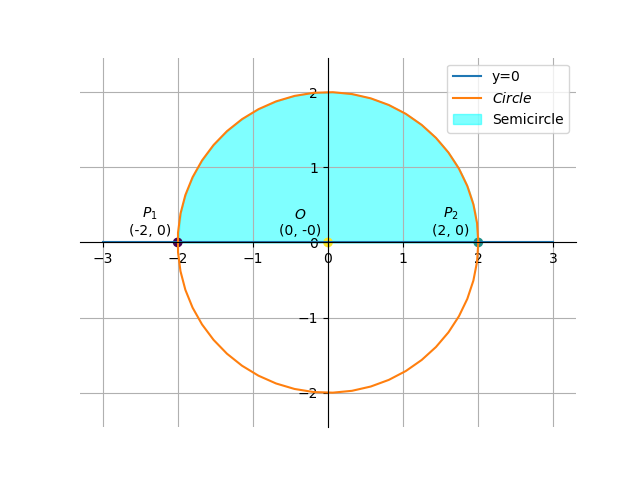
\includegraphics[scale=0.5]{plot}
    \caption{}
    \label{fig:plot}
\end{figure}
\end{document}
